%\documentclass[landscape,a0paper,fontscale=0.285]{baposter} % a0 is 841mm x 1189mm
\documentclass[landscape,archE,fontscale=0.285]{baposter} % archE is 36in x 48in

% Define colors from UT web page
\selectcolormodel{RGB}
%\definecolor{utburntorange}{cmyk}{0,0.2549,0.3922,0.03529}
\definecolor{burntorange}{RGB}{191,87,0}
\definecolor{rightfooterorange}{RGB}{248,151,31}
\definecolor{pms432}{RGB}{51,63,72}
\definecolor{pms7469}{RGB}{0,95,134}
\definecolor{pms7572}{RGB}{214,210,196}
\definecolor{pms7543}{RGB}{156,173,183}


\usepackage{graphicx} % Required for including images
\graphicspath{{../fig}}

\usepackage{graphbox}
\usepackage{overpic}
\usepackage[caption=false]{subfig}

\usepackage{hyperref}
\hypersetup{
  colorlinks=true,
  urlcolor=pms432,
  pdftitle={Pecos Poster Template},
}

\usepackage{listings}
\lstset{numbers=left,
  basicstyle=\tiny\ttfamily,
  keywordstyle=\color{blue},
  breaklines=true,
  showtabs=false,
  showstringspaces=false,
  xleftmargin=2.5em,
}

\usepackage{amsmath} % For typesetting math
\usepackage{amssymb} % Adds new symbols to be used in math mode

\usepackage{booktabs} % Top and bottom rules for tables
\usepackage{enumitem} % Used to reduce itemize/enumerate spacing
\usepackage{palatino} % Use the Palatino font
\usepackage[font=small,labelfont=bf]{caption} % Required for specifying captions to tables and figures

\usepackage{multicol} % Required for multiple columns
\setlength{\columnsep}{1.5em} % Slightly increase the space between columns
\setlength{\columnseprule}{0mm} % No horizontal rule between columns

\usepackage{tikz} % Required for flow chart
\usetikzlibrary{shapes,arrows} % Tikz libraries required for the flow chart in the template

\newcommand{\compresslist}{ % Define a command to reduce spacing within itemize/enumerate environments, this is used right after \begin{itemize} or \begin{enumerate}
\setlength{\itemsep}{1pt}
\setlength{\parskip}{0pt}
\setlength{\parsep}{0pt}
}
\newcommand{\overbar}[1]{\mkern 1.5mu\overline{\mkern-1.5mu#1\mkern-1.5mu}\mkern 1.5mu}
\newcommand{\pp}[2]{\frac{\partial #1}{\partial #2}}
\newcommand{\dd}[2]{\frac{d #1}{d #2}}
\newcommand{\DD}[2]{\frac{D #1}{D #2}}
\newcommand{\mm}{\mathbf{minmod}}
\def\etal{{\it et al~}}
\newcommand{\be}{\begin{eqnarray}}
	\newcommand{\ee}{\end{eqnarray}}
\newcommand{\mbb}[1]{\mathbb{#1}} % math blackboard bold
\newcommand{\mcal}[1]{\mathcal{#1}} % math blackboard bold
\newcommand{\mbf}[1]{\mathbf{#1}} % math bold face (for vectors)
\newcommand{\sbf}[1]{\boldsymbol{#1}} % bold face for symbols
\newcommand{\jump}[1]{\llbracket #1 \rrbracket} % jump operator
\newcommand{\avg}[1]{\langle #1 \rangle} % average operator
\newcommand{\rarrow}{\rightarrow}
\newcommand{\Rarrow}{\Rightarrow}
\newcommand{\LRarrow}{\Leftrightarrow}
\newcommand{\vvvert}{|\kern-1pt|\kern-1pt|}
\newcommand{\enorm}[1]{\vvvert #1 \vvvert}
\newcommand{\nutil}{\tilde{\nu}}
\newcommand{\Var}{\mathrm{Var}}
\newcommand{\Cov}{\mathrm{Cov}}


\definecolor{MyDarkGreen}{rgb}{0,0.45,0.08}
\newcommand{\myred}[1]{{\color{red} #1}}
\newcommand{\myblue}[1]{{\color{blue} #1}}
\newcommand{\mygreen}[1]{{\color{MyDarkGreen} #1}}

\newcommand{\sa}{\nu_{\mathrm{sa}}}
\newcommand{\tep}{\tilde{\epsilon}}
\newcommand{\Ssd}{\mathcal{S}} % source term due to slow derivative
\newcommand{\ud}{\,\mathrm{d}}

\newcommand{\Mach}[1]{\ensuremath{\mbox{Ma}_{#1}}}
\newcommand{\Reynolds}{\ensuremath{\mathit{Re}}}
\newcommand{\DensityRat}{\ensuremath{\mathit{DR}}}
\newcommand{\BlowRat}{\ensuremath{\mbox{BR}}}
\newcommand{\VelRat}{\ensuremath{\mathit{VR}}}
\newcommand{\Tau}{\ensuremath{\mathrm{T}}}

\newcommand{\wall}     {\ensuremath{\mathrm{w}}}   % wall subindex
\newcommand{\awall}    {\ensuremath{\mathrm{aw}}}  % adiabatic wall subindex

\newcommand{\commentout}[1]{}

\newcommand{\vect}[1]{\boldsymbol{#1}}
\usepackage{mleftright}
\newcommand{\of}[1]{\mleft( #1 \mright)}
\newcommand{\vth}{v_{\textrm{th}}}
\newcommand{\reals}{\mathbb{R}}
\newcommand{\myint}{\int\limits}
\newcommand{\ddt}[1]{\partial_t #1}
\newcommand{\RR}{\mathbb{R}}
\newcommand{\vr}{v}
\newcommand{\diff}[1]{\, d#1}
\newcommand{\norm}[1]{\left\lVert#1\right\rVert}
%\newcommand{\vtheta}{\theta_{\vect{v}}}
%\newcommand{\vphi}{\varphi_{\vect{v}}}
%\newcommand{\vr}{v_{r}}
\newcommand{\vtheta}{v_{\theta}}
\newcommand{\vphi}{v_{\varphi}}
\newcommand{\vomega}{v_{\omega}}
\newcommand{\vrunit}{\hat{\vect{v}}_{r}}
\newcommand{\vthetaunit}{\hat{\vect{v}}_{\theta}}
\newcommand{\vphiunit}{\hat{\vect{v}}_{\varphi}}
\DeclareMathOperator{\variance}{Var}


\begin{document}

\begin{poster}
{
columns=4, % number of columns (change to suite your needs)
headerborder=closed, % Adds a border around the header of content boxes
colspacing=1em, % Column spacing
bgColorOne=white, % Background color for the gradient on the left side of the poster
bgColorTwo=white, % Background color for the gradient on the right side of the poster
borderColor=burntorange, % Border color
headershade=plain,
headerColorOne=burntorange, % Background color for the header in the content boxes (left side)
headerColorTwo=burntorange, %burntorange, % Background color for the header in the content boxes (right side)
headerFontColor=white, % Text color for the header text in the content boxes
boxColorOne=white, % Background color of the content boxes
textborder=roundedleft, % Format of the border around content boxes, can be: none, bars, coils, triangles, rectangle, rounded, roundedsmall, roundedright or faded
eyecatcher=false, %true, % Set to false for ignoring the left logo in the title and move the title left
headerheight=0.09\textheight, % Height of the header
headershape=roundedright, % Specify the rounded corner in the content box headers, can be: rectangle, small-rounded, roundedright, roundedleft or rounded
headerfont=\Large\bf\textsc, % Large, bold and sans serif font in the headers of content boxes
%textfont={\setlength{\parindent}{1.5em}}, % Uncomment for paragraph indentation
linewidth=2pt % Width of the border lines around content boxes
}
%----------------------------------------------------------------------------------------
% TITLE SECTION (spans whole width)
%----------------------------------------------------------------------------------------
%
{}
{\bf\textsc{Solving the Boltzmann equation for electron kinetics using the Galerkin approach}\vspace{0.01em}} % Poster title
{\textsc{\small Milinda Fernando, Daniil Bochkov, Todd Oliver, Laxminarayan Raja, Philip Varghese, Robert Moser, and George Biros \hspace{12pt} \\The University of Texas at Austin}} % Author names and institution
{\includegraphics[align=c,height=0.09\textheight]{road_map.png}% just figure (must edit fig to add highlight box)
%\raisebox{-0.5\height}{\begin{overpic}[height=0.09\textheight]{pecos_roadmap_tst_1.5.pdf} % figure + highlight box
%    \put(-1,8){\filldraw [semithick, fill=rightfooterorange, fill opacity=0.1, draw=gray, rounded corners] (1.9,1.2) rectangle +(1.15,0.7);}
%\end{overpic}}%
\hspace{12pt} \includegraphics[align=c,height=3em]{psaap3-logo.png}%
\hspace{12pt} \includegraphics[align=c,height=3em]{oden_pecos_2020_wordmark.png}%
}

%----------------------------------------------------------------------------------------
%	OBJECTIVES
%----------------------------------------------------------------------------------------

\headerbox{Objectives}{name=objectives,column=0,row=0}{
\begin{itemize}
	\item \textbf{\textcolor{orange}{Main}}: Develop scalable robust deterministic Boltzmann solver to determine species kinetics properties to enable accurate plasma simulations. 
	\item \textbf{\textcolor{orange}{Representation}}: Identify robust, yet low cost efficient representation of the distribution function $f(t, \vect{v}, \vect{x})$.
	\item \textbf{\textcolor{orange}{Challenges}}: Dimensionality of the problem (6 + 1 dimensions), numerical + HPC challenges.
\end{itemize}
\vspace{0.3em} % When there are two boxes, some whitespace may need to be added if the one on the right has more content
}

%----------------------------------------------------------------------------------------
%	INTRODUCTION
%----------------------------------------------------------------------------------------

\headerbox{Introduction}{name=introduction,column=1,row=0}{
\begin{itemize}
	\item Electron distribution function $f\of{t,\vect{v}, \vect{x}}$ defines the transport and kinetic properties.
	\item Evolution of $f$ is described by the Boltzmann equation.
	\begin{align}
		\partial_t f + \vect{v}\cdot \nabla_{\vect{x}} f  - \frac{\vect{E} q}{m} \cdot \nabla_{\vect{v }}f = C(f)
	\end{align}
	\item Electric field $\vect{E}$ causes acceleration in the velocity space, and spatial advection occurs along $\vect{v}$, while the collision operator $C$ describes the underlying collisions. 
\end{itemize}
}

\headerbox{Methodology - 0D3V Boltzmann}{name=method,column=0,span=2,below=objectives}{ % This block's bottom aligns with the bottom of the conclusion block
	\begin{multicols}{2}
		\subsubsection*{Discretization}
		\begin{itemize}
			\item Weak formulation.\\
			$
			% \displaystyle
			% \quad
			\partial_t f - \frac{\vect{E} q}{m} \cdot \nabla_{\vect{v}}f = C(f)$
			$
			\Rightarrow 
			\partial_t \myint_{R^3} f \phi\of{\vect{v}} \ud \vect{v} = \myint_{R^3} C(f) \phi\of{\vect{v}} \ud \vect{v}$
			$\quad + \myint_{R^3} \of{\frac{\vect{E} q}{m} \cdot \nabla_{\vect{v}} f} \phi(\vect{v}) \ud \vect{v}$
			\item $f$ is approximated as isotropic + anisotropic correction terms.\\
			$
			% \displaystyle
			% \quad 
			f(\vect{v},t) = M(v)\sum_{klm} f_{klm} \Phi_k\of{v} Y_{lm}\of{v_\theta, v_\phi}$
			$ 
			% \displaystyle
			% \quad 
			\text{ with }
			\phi_{pqs}\of{\vect{v}} = \underbrace{\Phi_p\of{v}}_{\text{radial basis}} \underbrace{Y_{qs}\of{v_\theta, v_\phi}}_{\tiny\text{sph. harm.}}$
			\item Collision operator in weak form \\
			$
			% \displaystyle
			% \quad 
			% \small
			\myint_{R^3} C \phi\of{\vect{v}_e} \diff{\vect{v}_e} 
			=
			n_0 \myint_{R^3} \myint_{S^2} 
			B\of{\vect{v}_e, 0, \vect{\omega}} 
			f_e\of{\vect{v}_e} \times $ \\
			\text{\ \ \ \ \ \ \ \ \ } $
			\left(
			\phi\of{\vect{v}_e^\text{post}\of{\vect{v}_e, 0, \vect{\omega}}} 
			- \phi\of{\vect{v}_e} 
			\right)
			\diff{\vect{v}_e} \diff{\vect{\omega}}
			$
		\end{itemize}
		\subsubsection*{Steady-state solutions}
		\begin{itemize}
			\item Electric field accelerate electrons (adds energy), while collision causes energy loss.
			\item The normalized distribution function $\hat{f}\of{\vect{v},t}$ should reach a steady state.\\
			%\item We can directly solve the above to compute the steady-state solution.\\
			$
			% \displaystyle
			% \quad
			\partial_t (\hat{f}) = 0 \Rightarrow -(u^T C \hat{f}) \hat{f} + (C+E)\hat{f} =0
			$% with $u^T \hat{f}-1=0$
		\end{itemize}
		\columnbreak
		\subsubsection*{Simplified collision operator}
		\begin{itemize}
			%  \item For the moment assume lm=(0,0), (1,0) modes, %(i.e., two term expansion of distribution function)
			%  $
			%  % \displaystyle
			%  % \quad
			%  \vect{v}^{\prime} = (v_r^\prime, v_\theta^\prime, v_\phi^\prime) =\vect{v}^{post}\of{\vect{v},\vect{\omega}}$\\
			%  $
			%  % \displaystyle
			%  % \quad
			%  \cos v_\theta^\prime = \cos v_\theta \cos\chi + \sin v_\theta \sin \chi \cos\of{v_\phi-\phi}
			%  $
			\item Analytically integrating out the angles, we can write 
			$
			%\displaystyle
			%\quad
			\myint_{v} C^{q0}_{l0}\of{f} \psi(v) dv  = $\\$n_0 \myint_{v} v^3 \sigma\of{v} f\of{v} \delta_{ql}
			\of{\psi\of{v^{post}}\delta_{q0} - \psi\of{v}} \diff{v}$
		\end{itemize}
		\subsubsection*{Steady-state solution for EEDF}
		\begin{itemize}
			\item Two term expansion projected onto sph. harmonics\\
			$
			\frac{d}{dt} f_{0,0} - E 
			\left( \frac{1}{\sqrt{3}} \frac{d}{d\vr} f_{1,0} 
			+  \frac{2}{\sqrt{3}} \frac{1}{\vr} f_{1,0} \right) = \tilde{C_0} f_{0,0}
			$
			$\frac{d}{dt} f_{1,0} - E 
			\left( \frac{1}{\sqrt{3}} \frac{d}{d\vr} f_{0,0} \right) =  \tilde{C_1} f_{1,0}
			$
			\item For steady state we can write, \\
			$\frac{E^2}{3} \partial_{v} \of{\frac{\partial_v \hat f_0}{(n_0 \varepsilon^{1/2}\gamma \sigma\of{\varepsilon} + \mu)}} + \frac{2E^2}{3v} \frac{\partial_v \hat{f_0}}{(n_0 \varepsilon^{1/2}\gamma \sigma\of{\varepsilon} + \mu)} + \tilde C_0 \hat{f_0} = \mu \hat{f_0}$\\
			$\hat{f_1} = \frac{E}{\sqrt{3}} \frac{\partial_{v}\hat{f_0}}{(n_0 \varepsilon^{1/2}\gamma \sigma\of{\varepsilon} + \mu)}$
			
		\end{itemize}
		\subsubsection*{Parallelization}
		\begin{itemize}
			\item Use \texttt{Cupy} to achieve single GPU parallelization. 
			\item \textbf{Multi-GPU}: Combine with MPI + Parla.  
		\end{itemize}
	\end{multicols}
}

%----------------------------------------------------------------------------------------
%	REFERENCES
%----------------------------------------------------------------------------------------

% \headerbox{References}{name=references,column=0,above=bottom}{

% \renewcommand{\section}[2]{\vskip 0.05em} % Get rid of the default "References" section title
% \nocite{*} % Insert publications even if they are not cited in the poster
% \small{ % Reduce the font size in this block
% \bibliographystyle{unsrt}
% \bibliography{sample} % Use sample.bib as the bibliography file
% }}

% %----------------------------------------------------------------------------------------
% %	FUTURE RESEARCH
% %----------------------------------------------------------------------------------------
\headerbox{1D Glow Discharge}{name=glow_discharge,column=2,span=1,row=0}{
\begin{center}
	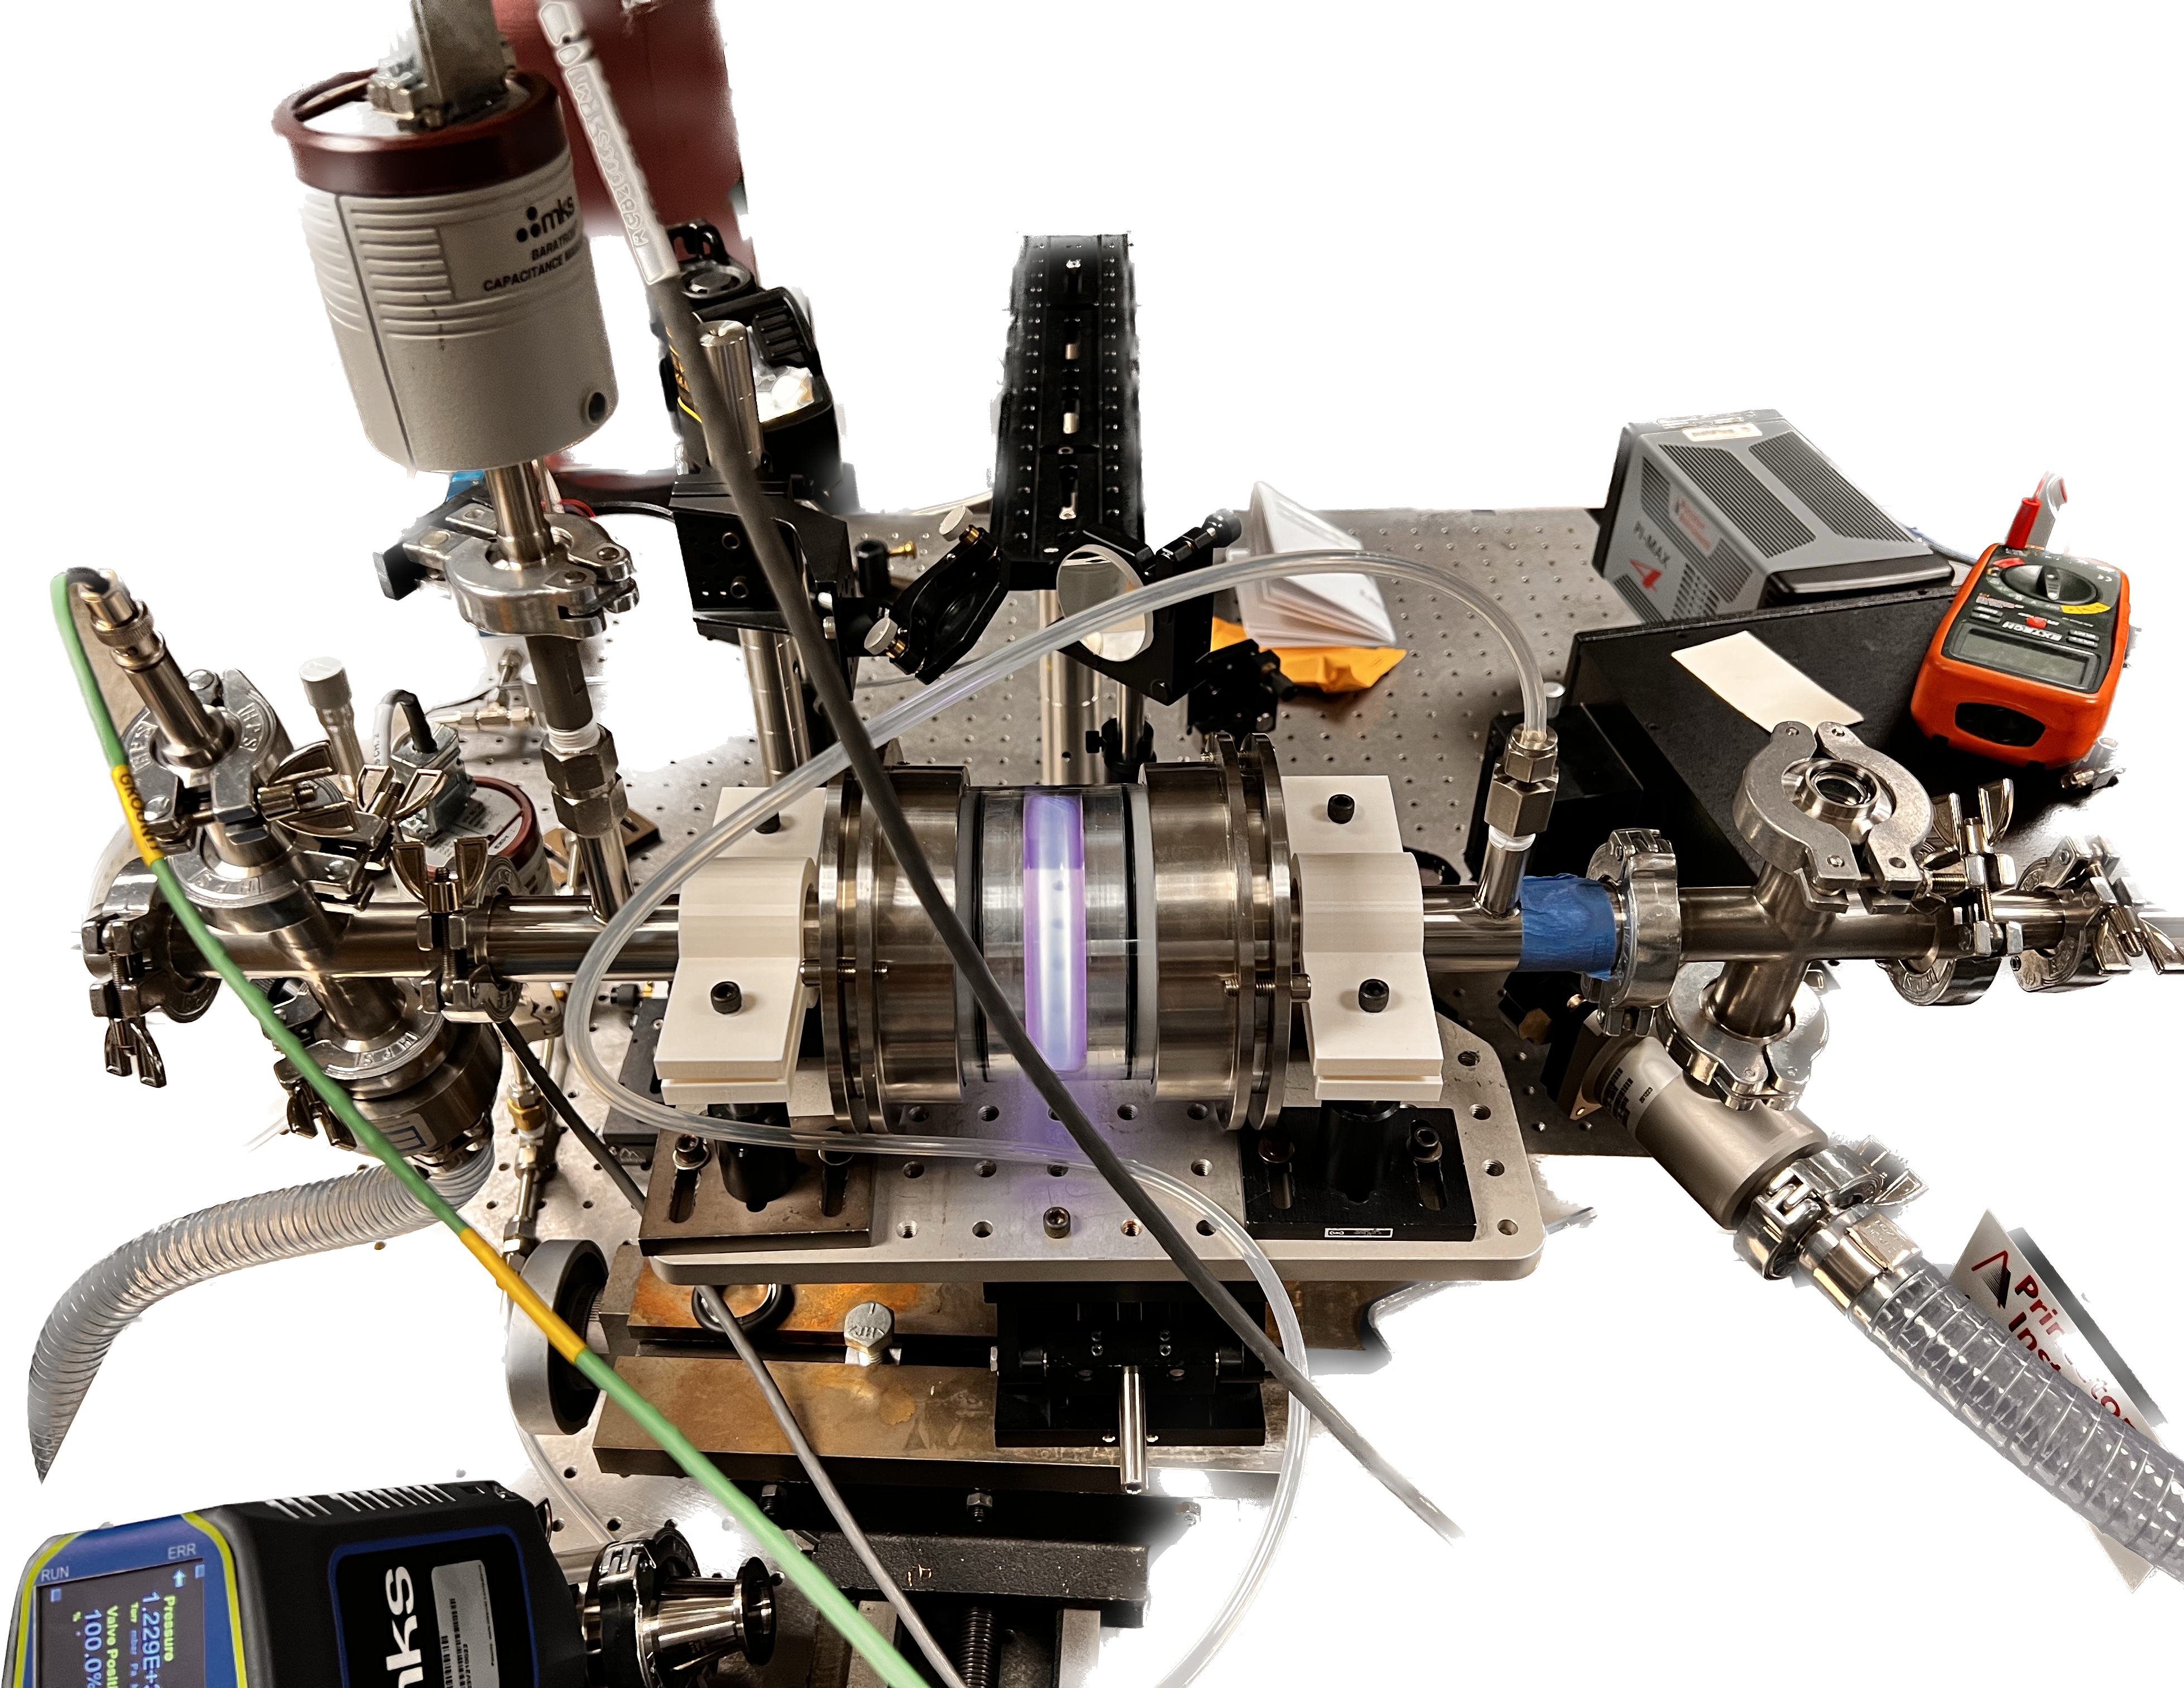
\includegraphics[width=0.7\textwidth]{eye-candy/glow/glow1.png}
\end{center}
\subsubsection*{Formulation}
\footnotesize{
\begin{align}
	&\partial_t f + v\cos\of{\vtheta} \partial_z f -\vect{E}\cdot\nabla_v f = C[f] \\
	&\textcolor{red!80}{f(\vect{v}, 0, t, \vtheta \leq \frac{\pi}{2})	= 0 \text{ and } f(\vect{v}, L, t, \vtheta > \frac{\pi}{2})	= 0}\\
	&\partial_t n_i + \partial_z \of{\mu_i n_i E\of{z,t} -D_i \partial_z n_i} = N \gamma \myint_{\varepsilon}\myint_{\vect{\omega}} \varepsilon^{1/2} \sigma_i f d\vect{\omega} d\varepsilon \\
	& \vect{E} = \nabla \of{\Delta^{-1}\frac{e}{\epsilon_0} \of{n_i- n_e}} \text{ , } n_e = \myint_{\vect{v}} f\of{\vect{v}, z, t} \diff{\vect{v}}
\end{align}}
\subsubsection*{Discretization}
\begin{itemize}
	\item Use method of discrete ordinates in $\vtheta$, $f_{\vtheta_j} = f(v, \vtheta_j, z, t)$
	\footnote{
	\begin{align}
		\partial_t f_{\vtheta_j} + v\cos\of{\vtheta_j} \partial_z f_{\vtheta_j} = P_{\vtheta_j} (C + E) \begin{bmatrix}
			f_{\vtheta_0}\\
			\vdots\\
			f_{\vtheta_{N_\vtheta}}\\
		\end{bmatrix} ; \\
		j=1,..., N_{\vtheta} \nonumber
	\end{align}}
	\item Use B-splines + spherical basis representation of $f$ in the velocity-space for collision and v-space advection
	\item Use finite difference method in $z$ direction
	\item Use method of lines + with explicit time integrator in time
	\item First order explicit operator splitting for evolving $n_i$ and $\vect{E}$ field equations
\end{itemize}
}

\headerbox{Future Work}{name=future_work,column=2,span=1,row=0,below=glow_discharge,above=bottom}{
	\begin{itemize}
	\item Add filtering in $\vtheta$ direction
	\item Supports adaptive discrete ordinates in space
	\item Integration with PyKokos and Parla
	\item Revisit radial discretization
	\begin{itemize}
		\item DG or finite volume discretization
	\end{itemize}
	%\item Artificial diffusion in speed, for stabilization ?
\end{itemize}
}


%----------------------------------------------------------------------------------------
%	CONTACT INFORMATION
%----------------------------------------------------------------------------------------

%%% \headerbox{Contact Information}{name=contact,column=3,aligned=references,above=bottom}{ % This block is as tall as the references block
%%% \begin{description}\compresslist
%%% \item[Web] www.university.edu/smithlab
%%% \item[Email] john@smith.com
%%% \end{description}
%%% }

%----------------------------------------------------------------------------------------
%	CONCLUSION
%----------------------------------------------------------------------------------------

\headerbox{Conclusions}{name=conclusions,column=0,span=2,below=method,above=bottom}{ % This block is as tall as the references block
\begin{itemize}
  \item Diffusion helps to stabilize tail oscillations and accurate tail representation.
  \item Global polynomials (Maxwell, and others) have spectral convergence, yet struggle to represent tails in the presence of sharp variations. 
  \item Local approximations provide a flexible framework to capture the tails comparatively better compared to global approximations. 
\end{itemize}
}

%----------------------------------------------------------------------------------------
%	RESULTS 1
%----------------------------------------------------------------------------------------

\headerbox{Results - 0D3V Boltzmann}{name=results_0d3v,column=3,span=1,row=0}{
	\subsubsection*{Global vs. Local Galerkin approximations}
	\begin{center}
		\includegraphics[width=\textwidth]{maxwell_E200_g0g2.png}
		\vspace{-0.2in}
		\captionof{figure}{Maxwell polynomials (global)}
	\end{center}
	\vspace{-0.2in}
	\begin{center}
		\includegraphics[width=\textwidth]{bspline_sp2_E200_g0g2.png}
		\vspace{-0.2in}
		\captionof{figure}{B-Splines (local)}
	\end{center}
	\vspace{-0.2in}
	\begin{center}
		\includegraphics[width=\textwidth]{bspline_sp2_E200_g0g2_eedf.png}
		\vspace{-0.2in}
		\captionof{figure}{B-Splines + EEDF formulation}
	\end{center}
	\vspace{-0.2in}
	\subsubsection*{Validation with Bolsig+ code}
	\begin{center}
		\includegraphics[width=\textwidth]{pde_vs_bolsig_collop_approx_eedf.png}
		\vspace{-0.2in}
		\captionof{figure}{Verification results with Bolsig+}
	\end{center}
}

\headerbox{Results - 1D3V Boltzmann}{name=results_1d3v,column=3,span=1,row=0,above=bottom,below=results_0d3v}{
	\subsubsection*{1D Glow Discharge with Boltzmann}
	\begin{center}
		\includegraphics[width=\textwidth]{glow_discharge_1d3v_g0_g2_v0_z01.0_E0.0_poly_bspline_sp_2_nr128_lmax3_qpn4_ev2.000000E+00_bscale1.0_dt1.0000E-13_T1.00E-10_qoi.png}
		\captionof{figure}{1D glow discharge with Boltzmann equation}
	\end{center}

}

%----------------------------------------------------------------------------------------
%	MATERIALS AND METHODS
%----------------------------------------------------------------------------------------



%----------------------------------------------------------------------------------------
%	RESULTS 2
%----------------------------------------------------------------------------------------

% \headerbox{Results 2}{name=results2,column=1,below=objectives,bottomaligned=conclusion}{ % This block's bottom aligns with the bottom of the conclusion block

% Donec faucibus purus at tortor egestas eu fermentum dolor facilisis. Maecenas tempor dui eu neque fringilla rutrum. Mauris \emph{lobortis} nisl accumsan.

% \begin{center}
% \begin{tabular}{l l l}
% \toprule
% \textbf{Treatments} & \textbf{Response 1} & \textbf{Response 2}\\
% \midrule
% Treatment 1 & 0.0003262 & 0.562 \\
% Treatment 2 & 0.0015681 & 0.910 \\
% Treatment 3 & 0.0009271 & 0.296 \\
% \bottomrule
% \end{tabular}
% \captionof{table}{Table caption}
% \end{center}

% Nulla ut porttitor enim. Suspendisse venenatis dui eget eros gravida tempor. Mauris feugiat elit et augue placerat ultrices. Morbi accumsan enim nec tortor consectetur non commodo.

% \begin{center}
% \begin{tabular}{l l l}
% \toprule
% \textbf{Treatments} & \textbf{Response 1} & \textbf{Response 2}\\
% \midrule
% Treatment 1 & 0.0003262 & 0.562 \\
% Treatment 2 & 0.0015681 & 0.910 \\
% Treatment 3 & 0.0009271 & 0.296 \\
% \bottomrule
% \end{tabular}
% \captionof{table}{Table caption}
% \end{center}
% }

%----------------------------------------------------------------------------------------

\end{poster}

\end{document}
